% appendix_a.tex

\chapter{Zusätzliche Daten und Informationen}
\label{appendix_a}

\section{Erstellung eines flexiblen Interfaces mit FastAPI und Swagger}

Mit \texttt{FastAPI} und \texttt{Swagger} lässt sich ein flexibles und interaktives API-Interface für das 
Framework erstellen, das eine umfassende Dokumentation sowie effiziente Testmöglichkeiten bereitstellt.
Siehe Abbilung \ref{fig:Swagger_UI} für eine Darstellung der \textit{Swagger UI}.

\section{benutzerfreundliche Interface, um das Framework zu testen}

Beispiel für eine benutzerfreundliche Oberfläche, um das Framework zu testen und die API-Endpunkte zu überprüfen.

\section{Vergleich von Optimierungstechniken für ML-Modelle}

In Tabelle \ref{tab:appendix_table} wird ein Vergleich verschiedener Optimierungstechniken für Machine-Learning-Modelle.


\begin{figure}[h!]
    \centering
    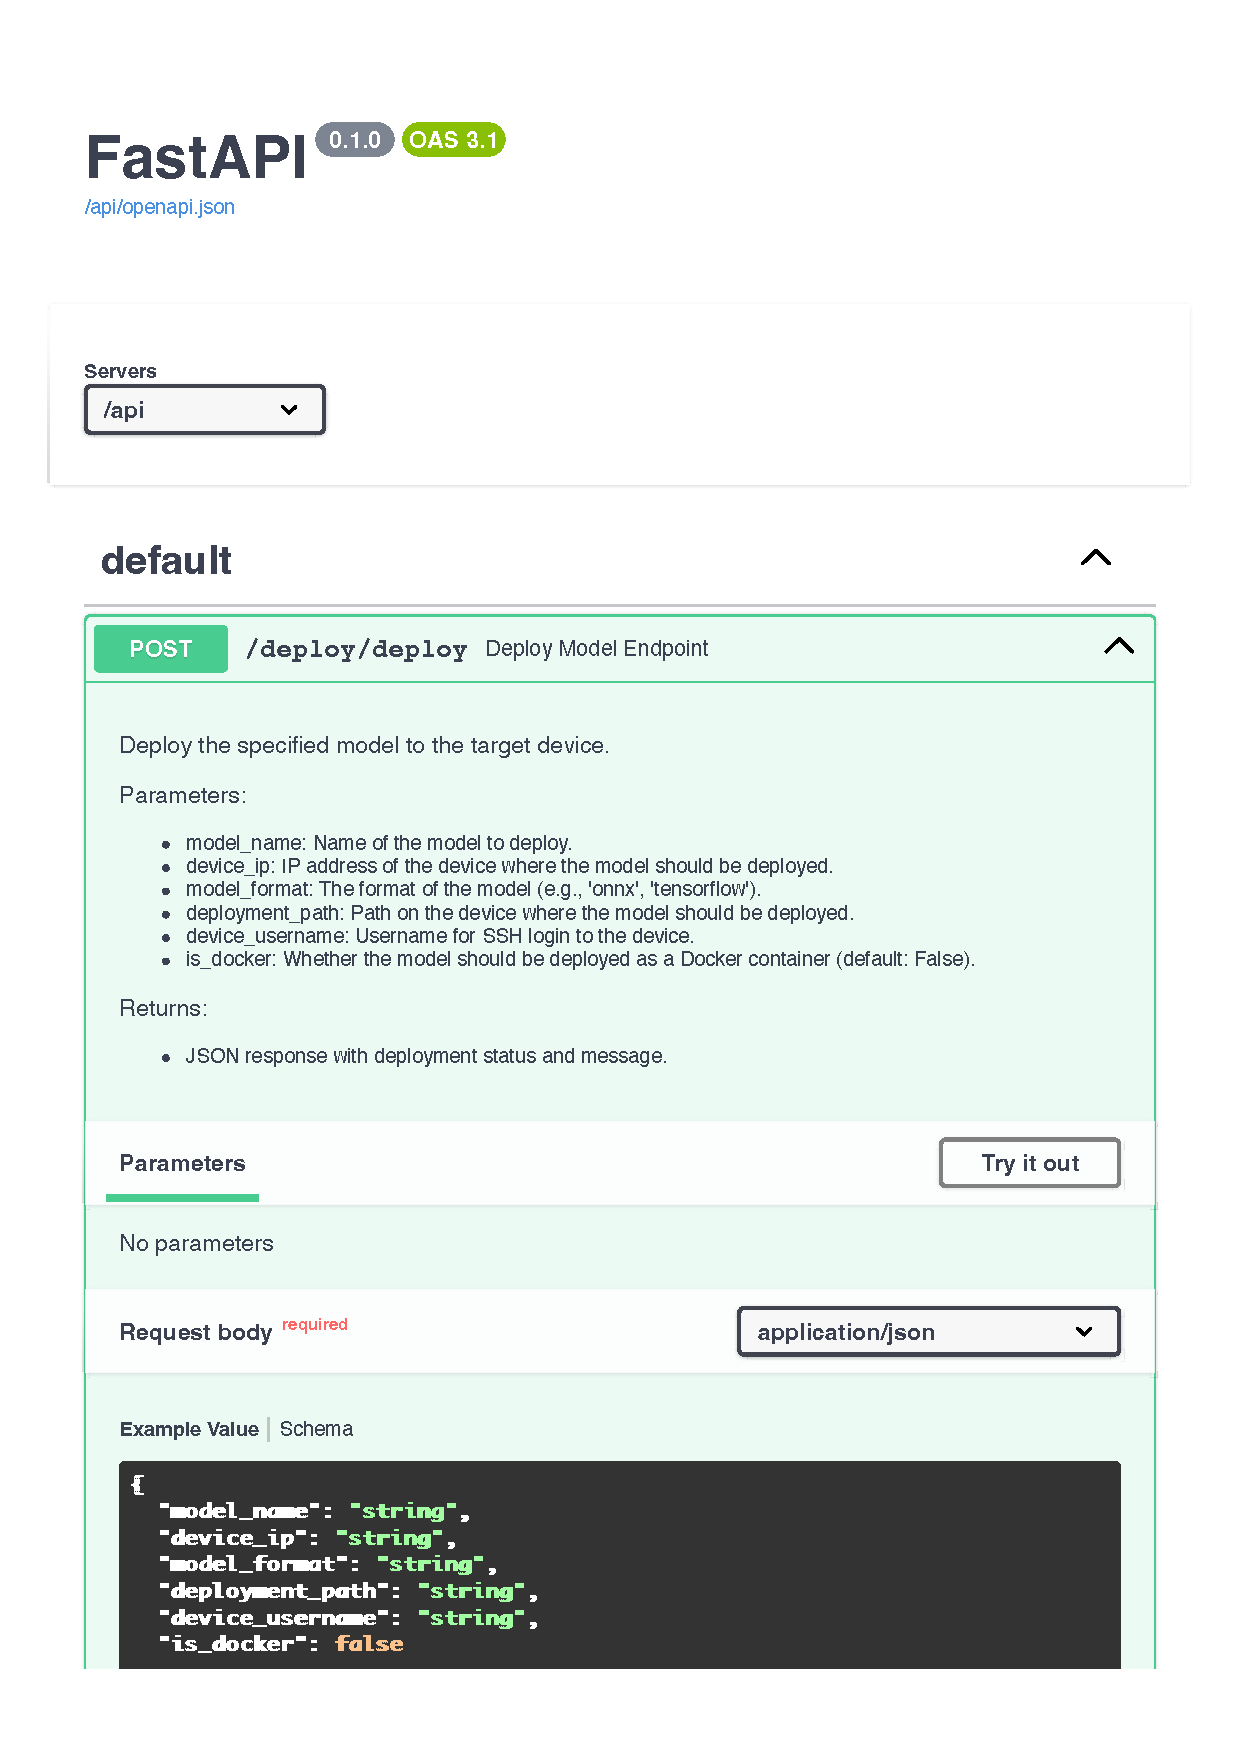
\includegraphics[width=1\textwidth]{FastAPI_Swagger_UI.pdf} 
    \caption{Framework-API mit Swagger UI} 
    \label{fig:Swagger_UI} 
\end{figure}


\begin{sidewaystable}[h!]
    \centering
    \caption{Vergleich von Optimierungstechniken für ML-Modelle}
    \begin{tabular}{|l|p{4cm}|p{4cm}|p{4cm}|p{4cm}|}
    \hline
    \textbf{Optimierungstechnik} & \textbf{Modellgröße} & \textbf{Effizienz (Latenz/Durchsatz)} & \textbf{Einfluss auf Genauigkeit} & \textbf{Anwendungsbeispiel} \\ \hline
    \textbf{Quantisierung} & Reduziert Speicherbedarf stark (durch Umwandlung in 8-Bit-Ganzzahlen) & Signifikant verbessert, besonders bei Inferenzzeiten & Geringer Einfluss bei sorgfältiger Anwendung, besonders mit Quantization-Aware Training & Mikrocontroller und Systeme mit geringer Rechenleistung \\ \hline
    \textbf{Pruning} & Reduziert Größe durch Entfernen unnötiger Verbindungen & Effizienz verbessert, aber erfordert zusätzliche Schritte im Training & Minimaler Einfluss bei unstrukturiertem Pruning; strukturiertes Pruning kann leicht die Genauigkeit senken & Tiefe neuronale Netze auf SPS und IPCs \\ \hline
    \textbf{Modellkompression} & Sehr effektive Reduktion redundanter Parameter, besonders bei großen Modellen & Effizienz gesteigert durch schnelleren Zugriff auf Speicher & Kaum signifikante Einbußen bei großen, komplexen Modellen & Edge-Devices und Systeme mit variierenden Speicheranforderungen \\ \hline
    \textbf{Knowledge Distillation} & Reduziert Größe erheblich, da komplexes Modell durch kleineres „Schülermodell“ ersetzt wird & Effizienz durch geringeren Speicherverbrauch und schnellere Berechnungen erhöht & Kann zu leichtem Genauigkeitsverlust führen; abhängig von der Distillation-Methode & Mobile Geräte und Echtzeitsysteme \\ \hline
    \textbf{Weight Clustering} & Mittlere Reduktion, da gleiche Gewichte gruppiert und komprimiert werden & Geringfügige Effizienzverbesserung & Bei grober Clusterung kann die Genauigkeit leiden & Geringfügig ressourcenbeschränkte Systeme \\ \hline
    \end{tabular}
    \label{tab:appendix_table}
\end{sidewaystable}

\begin{figure}[h!]
    \centering
    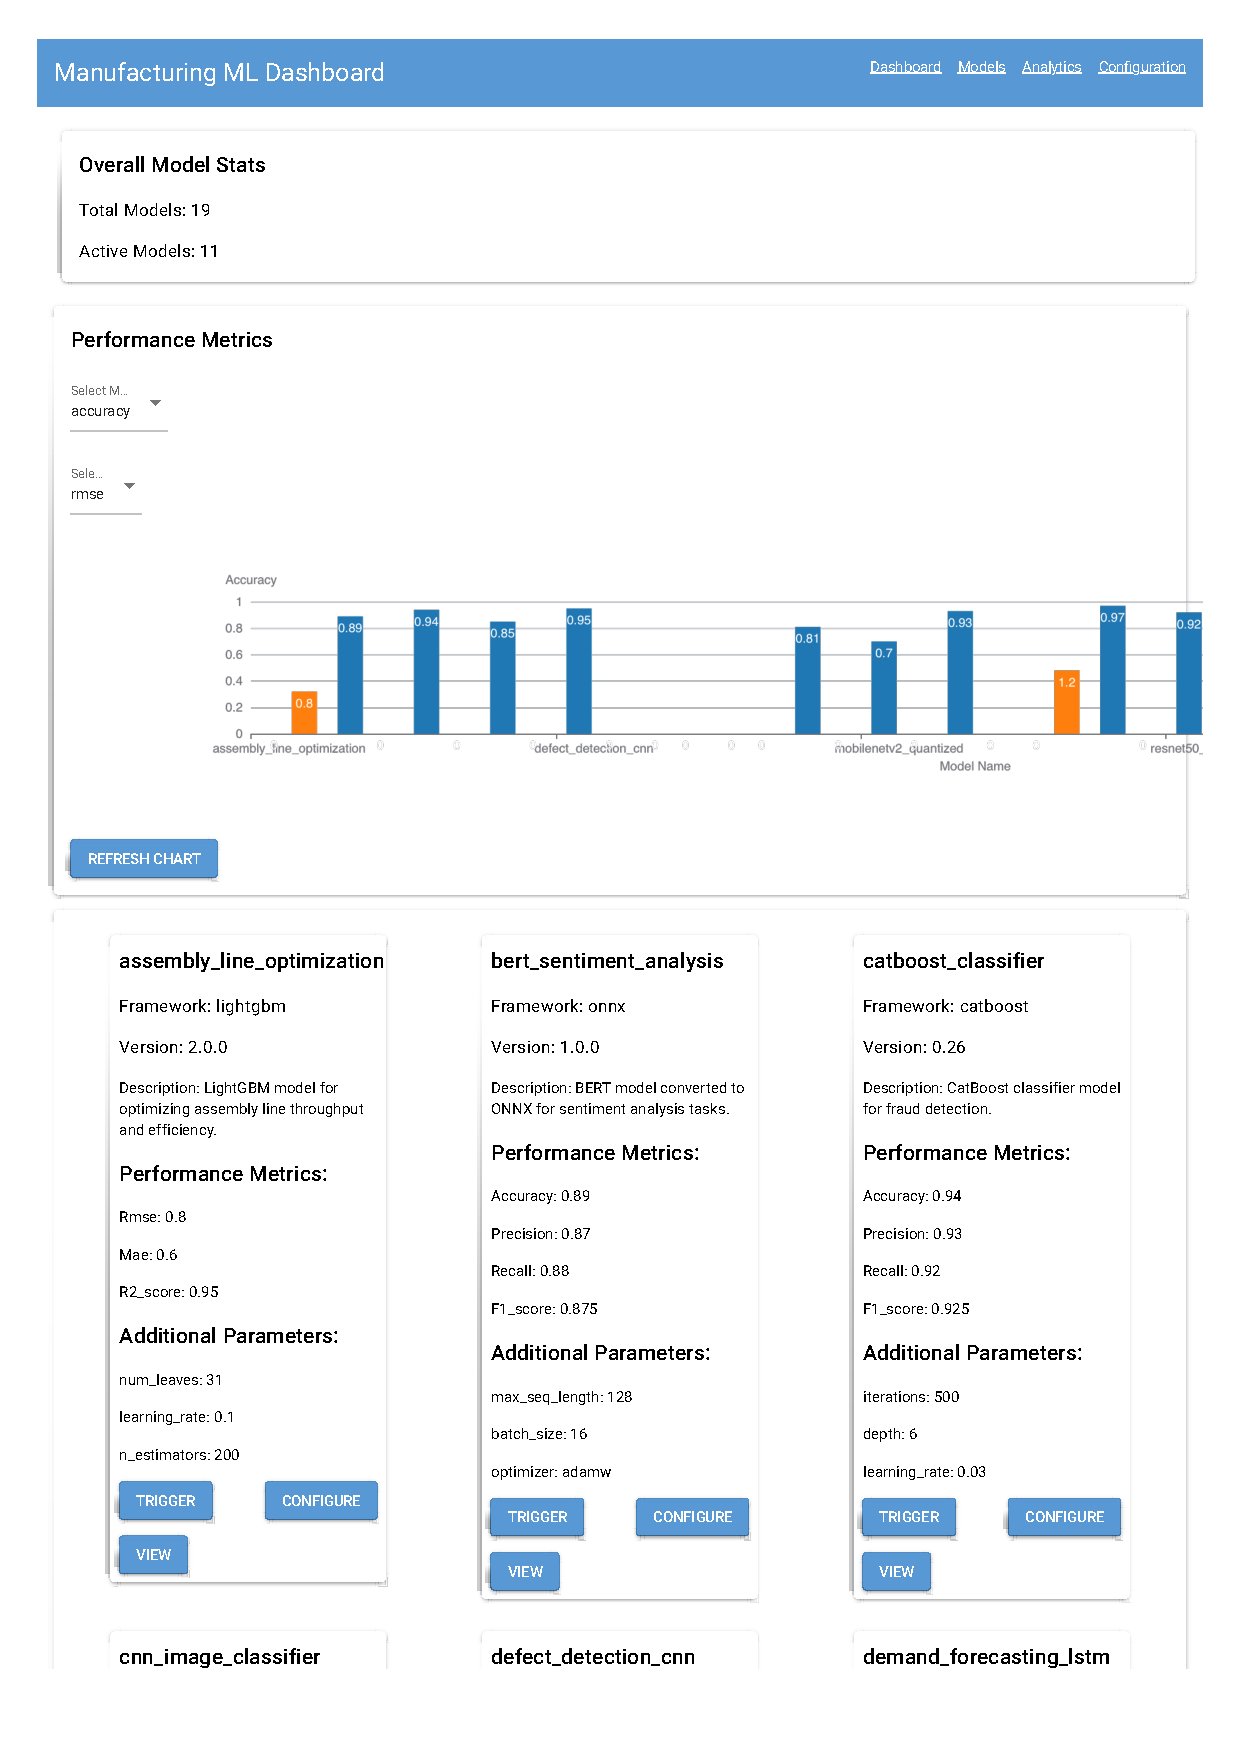
\includegraphics[width=1\textwidth]{NiceGuiModelsInformation.pdf} 
    \caption{Übersicht über verfügbare ML-Modelle} 
    \label{fig:NiceGUI_Models}
\end{figure}